\documentclass[conference]{IEEEtran}
\IEEEoverridecommandlockouts
% The preceding line is only needed to identify funding in the first footnote. If that is unneeded, please comment it out.
\usepackage{cite}
\usepackage{amsmath,amssymb,amsfonts}
\usepackage{algorithmic}
\usepackage{graphicx}
\usepackage{textcomp}
\usepackage{xcolor}
\usepackage{listings}
\usepackage{hyperref}
\usepackage{xparse}


\definecolor{mGreen}{rgb}{0,0.6,0}
\definecolor{mGray}{rgb}{0.5,0.5,0.5}
\definecolor{mPurple}{rgb}{0.58,0,0.82}
\definecolor{backgroundColour}{rgb}{0.95,0.95,0.92}

\NewDocumentCommand{\codeword}{v}{%
	\texttt{\textcolor{blue}{#1}}%
}

\lstdefinestyle{CStyle}{
	backgroundcolor=\color{backgroundColour},   
	commentstyle=\color{mGreen},
	keywordstyle=\color{magenta},
	numberstyle=\tiny\color{mGray},
	stringstyle=\color{mPurple},
	basicstyle=\footnotesize,
	breakatwhitespace=false,         
	breaklines=true,                 
	captionpos=b,                    
	keepspaces=true,                 
	numbers=left,                    
	numbersep=5pt,                  
	showspaces=false,                
	showstringspaces=false,
	showtabs=false,                  
	tabsize=2,
	language=C
}

\lstset{language=C,keywordstyle={\bfseries \color{blue}}}

\def\BibTeX{{\rm B\kern-.05em{\sc i\kern-.025em b}\kern-.08em
    T\kern-.1667em\lower.7ex\hbox{E}\kern-.125emX}}
\begin{document}

\title{Weather Clock\\
{\footnotesize \textsuperscript{*}Echtzeit Datendarstellung auf dem Display}
}

\author{\IEEEauthorblockN{1\textsuperscript{st} Imron Gamidli}
\IEEEauthorblockA{\textit{Internationale Ingenieurwissenschaften} \\
\textit{Hochschule Fulda}\\
Fulda, Deutschland \\
imron.gamidli@lt.hs-fulda.de}
\and
\IEEEauthorblockN{2\textsuperscript{nd} Hussain Ali}
\IEEEauthorblockA{\textit{Internationale Ingenieurwissenschaften} \\
	\textit{Hochschule Fulda}\\
	Fulda, Deutschland \\
	husain.ali@lt.hs-fulda.de}
}

\maketitle

\begin{abstract}

\end{abstract}

\begin{IEEEkeywords}
dht22, arduino, uno, 
\end{IEEEkeywords}

\section{DHT22 Sensor}

\subsection{Beschreibung}
Der DHT22 ist ein einfacher, preiswerter digitaler Temperatur- und Feuchtigkeitssensor. Er verwendet einen kapazitiven Feuchtigkeitssensor und einen Thermistor, um die Umgebungsluft zu messen, und spuckt ein digitales Signal auf dem Datenpin aus (keine analogen Eingangspins erforderlich). Er ist recht einfach zu bedienen, erfordert aber ein sorgfältiges Timing bei der Datenerfassung. Der einzige wirkliche Nachteil dieses Sensors ist, dass man nur alle 2 Sekunden neue Daten von ihm erhalten kann, so dass bei Verwendung unserer Bibliothek die Sensormesswerte bis zu 2 Sekunden alt sein können.

Verbinden Sie einfach den ersten Pin auf der linken Seite mit 3-5V Strom, den zweiten Pin mit Ihrem Dateneingangspin und den ganz rechten Pin mit Masse. Obwohl der Sensor ein einziges Kabel zum Senden von Daten verwendet, ist er nicht mit Dallas One Wire kompatibel! Wenn Sie mehrere Sensoren wünschen, muss jeder seinen eigenen Datenpin haben.

Im Vergleich zum DHT11 ist dieser Sensor präziser, genauer und funktioniert in einem größeren Temperatur-/Feuchtigkeitsbereich, ist aber auch größer und teurer.

Wird mit einem 4.7K - 10K Widerstand geliefert, den Sie als Pullup vom Daten-Pin zu VCC verwenden wollen.

\subsection{Technische Daten}
\begin{itemize}
	\item Geringe Kosten
	\item 3 bis 5V Stromversorgung und E/A
	\item Maximal 2,5 mA Stromverbrauch während der Umwandlung (während der Datenabfrage)
	\item Gut geeignet für 0-100% Luftfeuchtigkeit mit 2-5% Genauigkeit
	\item Gut geeignet für Temperaturmessungen von -40 bis 80°C mit einer Genauigkeit von ±0,5°C
	\item Abtastrate nicht mehr als 0,5 Hz (einmal alle 2 Sekunden)
	\item Gehäusegröße 27mm x 59mm x 13,5mm (1,05" x 2,32" x 0,53")
	\item 4 Stifte, 0,1" Abstand 
	\item Gewicht (nur der DHT22): 2,4g
\end{itemize}

	
\begin{figure}
	\begin{center}
		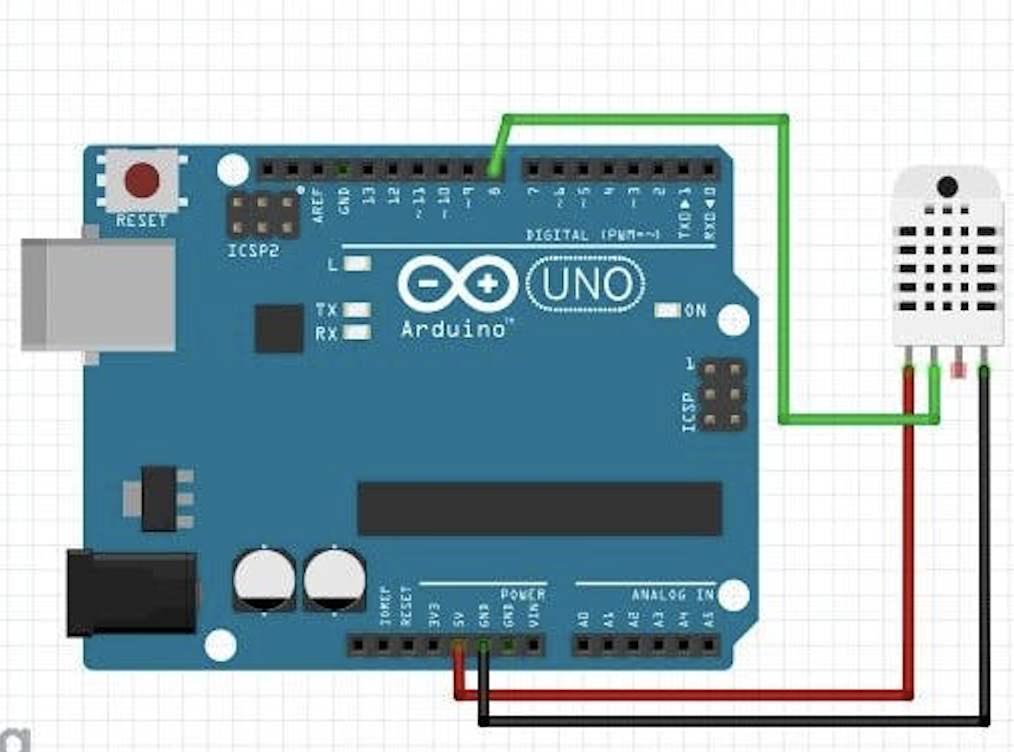
\includegraphics[scale=0.3]{dht22}
	\end{center}
	\caption{DHT22 Sensor}
\end{figure}

Es ist ziemlich einfach, die DHT-Sensoren anzuschließen. Sie haben vier Stifte VCC - roter Draht Schließen Sie an 3,3 - 5V Strom an. Manchmal reicht die 3,3-V-Spannung nicht aus, in diesem Fall versuchen Sie es mit einer 5-V-Spannung. Datenausgang - weißes oder gelbes Kabel Nicht angeschlossen Masse - schwarzes Kabel Ignorieren Sie einfach Pin 3, er wird nicht verwendet. Dieses Diagramm zeigt, wie wir für die Testskizze anschließen werden. Schließen Sie Daten an Pin 2 an, Sie können dies später auf jeden beliebigen Pin ändern.

\subsection{Implementierung im Projekt}
DHT22 war nützlich für unseres Projekt. Mithilfe diesen Sensor, bekommen wir Temperatur und Feuchtigkeit Daten. Damit es möglich wird, Sensordaten zu lesen, bestimmte Bibliothek muss installiert und importiert soll. Die Bibliothek für DHT22 heißt \textit{DHT sensor library} und installiert wurde vom \url{https://github.com/adafruit/DHT-sensor-library} . Nachdem wir die Bibliothek installiert haben, haben wir diese importiert.


\begin{lstlisting}[style=CStyle]
#include <DHT.h>;
\end{lstlisting}

Diese Bibliothek ermöglicht uns eine DHT Instanz initialisieren. Hier man sieht wir haben PIN 13 für DHT Kommunikation. Danach haben wir DHT22 Instanz erstellt.

\begin{lstlisting}[style=CStyle]
#define DHTPIN 13	// what pin we're connected to
#define DHTTYPE DHT22	// DHT 22 
DHT dht(DHTPIN, DHTTYPE);	// Initialize DHT 
\end{lstlisting}

Wir werden später Daten aus dem Sensor in Variablen speichern. Dafür haben wir zwei Variablen, \textsf{hum} für Feuchtigkeit und \textsf{temp} für Temperatur deklariert. 

\begin{lstlisting}[style=CStyle]
float hum;	//Stores humidity value
float temp;	//Stores temperature value
\end{lstlisting}

In \textsf{setup()} Funktion haben wir die DHT Instanz gestartet. Das heißt, die Instanz läuft und wir können jederzeit Feuchtigkeit und Temperaturdaten anfragen. 

\begin{lstlisting}[style=CStyle]
void setup()
{
	dht.begin();
}
\end{lstlisting}

In der Schleife \textsf{loop()} das Programm liest Feuchtigkeitswert mit \textsf{readHumidity()} und speichert in \textsf{hum} variable. Auf die gleiche Weise Temperatur wird mit \textsf{readTemperature()} gelesen und in \textsf{temp} gespeichert. 

\begin{lstlisting}[style=CStyle]
void loop()
{
	//Read data and store it to variables hum and temp
	hum = dht.readHumidity();
	temp = dht.readTemperature();
	
}
\end{lstlisting}

Letzte Aufgabe ist auf dem Display darzustellen, das vorher  mit entsprechender Adresse initialisiert wurde. Wir haben zwei Displays, für DHT Daten haben wir erste Reihe des erstens Display benutzt. 

\begin{lstlisting}[style=CStyle]
	void loop()
	{
		//Read data and store it to variables hum and temp
		hum = dht.readHumidity();
		temp = dht.readTemperature();
		
		lcd1.setCursor(0, 0);
		lcd1.print("tmp:");
		lcd1.print(temp); 
		lcd1.setCursor(6, 0);
		lcd1.print((char)223);
		lcd1.print("C hum:");
		lcd1.print(hum);
		lcd1.setCursor(15, 0);
		lcd1.print("%");
		
	}
\end{lstlisting}

\section{PIR Motion Sensor}
\subsection{Überblick}
PIR-Sensoren ermöglichen die Erfassung von Bewegungen und werden fast immer verwendet, um festzustellen, ob sich ein Mensch in den Sensorbereich hinein- oder herausbewegt hat. Sie sind klein, preiswert, stromsparend, einfach zu bedienen und verschleißen nicht. Aus diesem Grund werden sie häufig in Geräten und Vorrichtungen in Haushalten und Unternehmen eingesetzt. 
	
\begin{figure}
	\begin{center}
		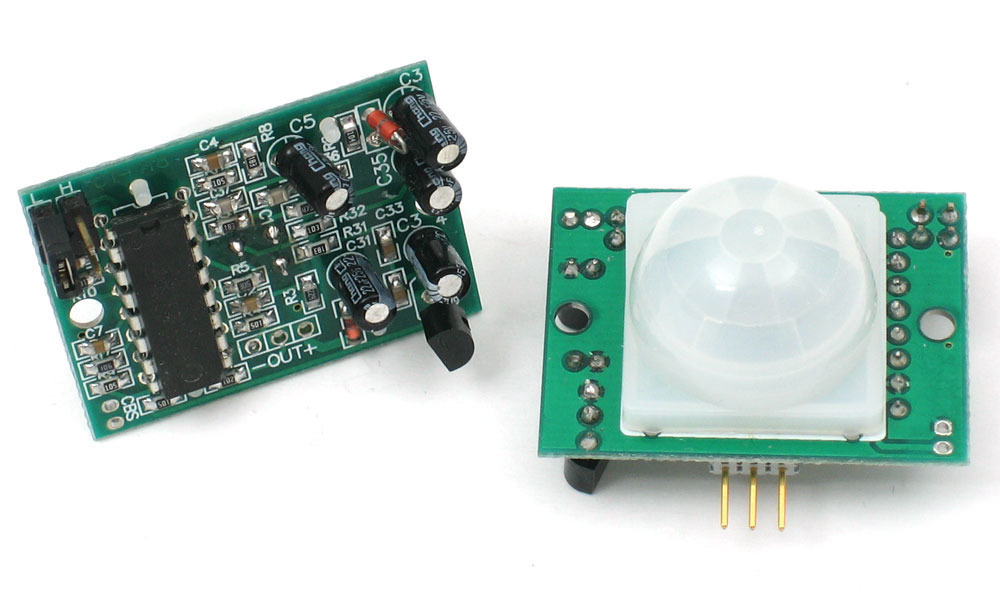
\includegraphics[scale=0.15]{pir1}
	\end{center}
	\caption{PIR Sensor}
\end{figure}

PIR-Sensoren bestehen im Wesentlichen aus einem pyroelektrischen Sensor (den Sie unten als runde Metalldose mit einem rechteckigen Kristall in der Mitte sehen können), der die Stärke der Infrarotstrahlung erkennen kann. Alles gibt eine schwache Strahlung ab, und je heißer etwas ist, desto mehr Strahlung wird freigesetzt. Der Sensor in einem Bewegungsmelder ist eigentlich in zwei Hälften geteilt. Der Grund dafür ist, dass wir eine Bewegung (Veränderung) und nicht die durchschnittliche IR-Stärke erkennen wollen. Die beiden Hälften sind so verdrahtet, dass sie sich gegenseitig aufheben. Wenn eine Hälfte mehr oder weniger IR-Strahlung sieht als die andere, schwankt der Ausgang nach oben oder unten.

\begin{figure}
	\begin{center}
		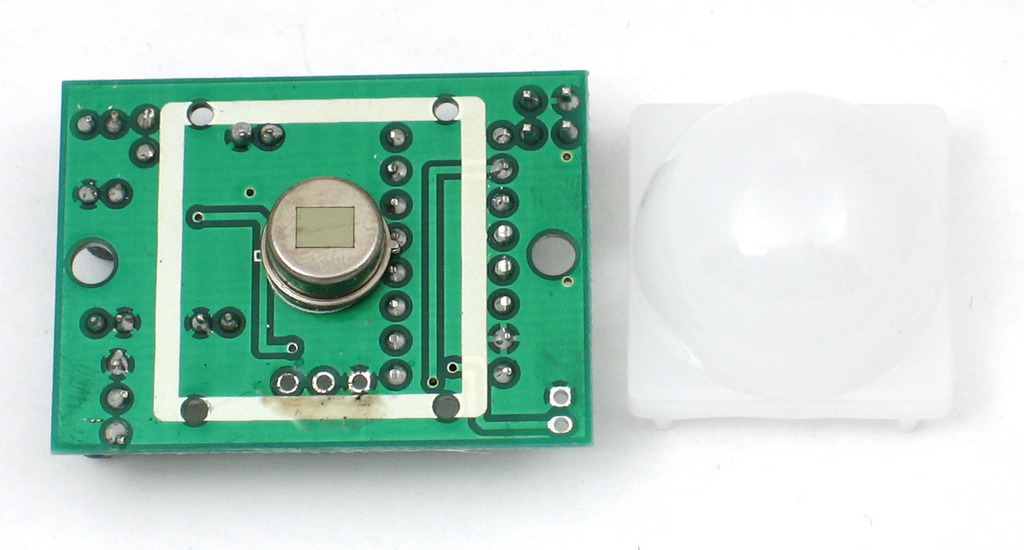
\includegraphics[scale=0.15]{pi2}
	\end{center}
	\caption{PIR Sensor 1}
\end{figure}

Zusammen mit dem pyroelektrischen Sensor gibt es eine Reihe von unterstützenden Schaltungen, Widerständen und Kondensatoren. Es scheint, dass die meisten kleinen Bastler-Sensoren den BISS0001 verwenden, zweifellos ein sehr preiswerter Chip. Dieser Chip nimmt das Ausgangssignal des Sensors auf und verarbeitet es ein wenig, um einen digitalen Ausgangsimpuls aus dem analogen Sensor zu erzeugen.

Im Vergleich zu älteren PIRs haben die neuen PIRs mehr einstellbare Einstellungen und sind mit einer Stiftleiste ausgestattet, die in den 3-poligen Masse-/Ausgangs-/Stromanschlüssen installiert ist.

\begin{figure}
	\begin{center}
		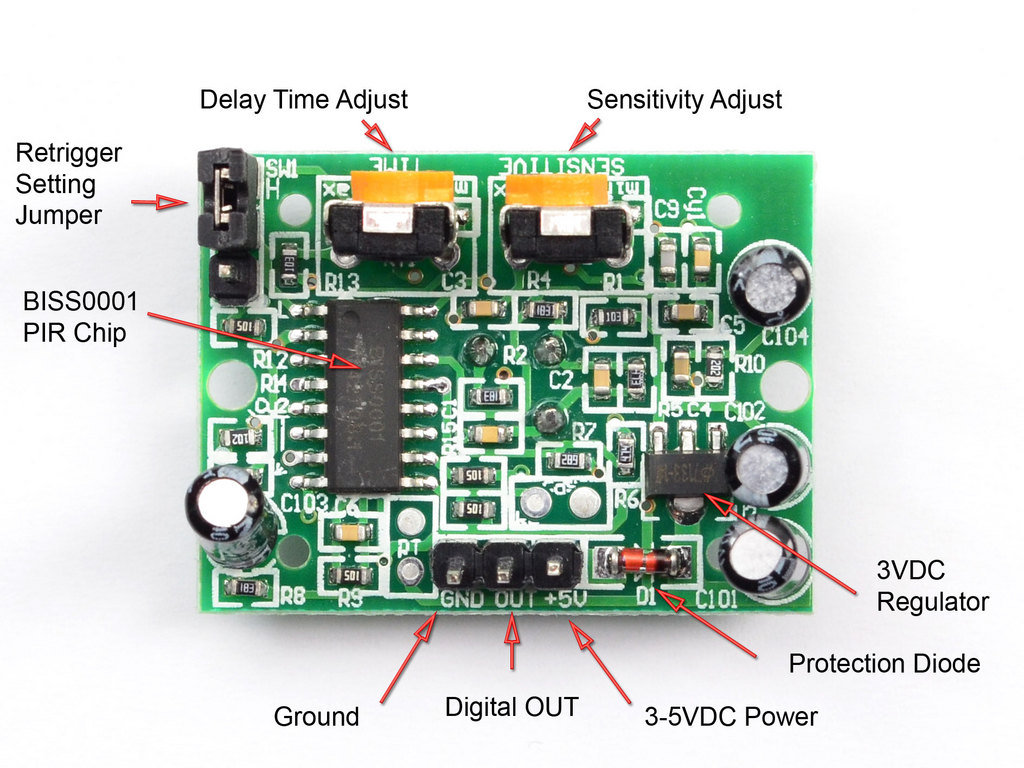
\includegraphics[scale=0.15]{pir3}
	\end{center}
	\caption{PIR Sensor Einstellungen}
\end{figure}

Für viele einfache Projekte oder Produkte, bei denen erkannt werden muss, ob eine Person den Bereich verlassen oder betreten hat oder sich ihm genähert hat, sind PIR-Sensoren hervorragend geeignet. Sie sind stromsparend und kostengünstig, ziemlich robust, haben einen großen Linsenbereich und sind einfach zu bedienen.  PIR-Sensoren zeigen nicht an, wie viele Personen sich in der Nähe aufhalten oder wie nah sie am Sensor sind. Die Linse ist oft auf einen bestimmten Bereich und eine bestimmte Entfernung festgelegt (obwohl sie irgendwo gehackt werden kann), und manchmal werden sie auch von Haustieren ausgelöst.

\subsection{Wie PIRs funktionieren}
PIR-Sensoren sind komplizierter als viele der anderen Sensoren, die in diesen Tutorials erklärt werden (wie Fotozellen, FSRs und Kippschalter), weil es mehrere Variablen gibt, die den Eingang und Ausgang des Sensors beeinflussen. Um zu erklären, wie ein grundlegender Sensor funktioniert, verwenden wir dieses schöne Diagramm

Der PIR-Sensor selbst hat zwei Schlitze. Jeder Schlitz besteht aus einem speziellen Material, das für IR empfindlich ist. Die Linse, die hier verwendet wird, macht nicht wirklich viel, und so sehen wir, dass die beiden Schlitze über eine gewisse Entfernung hinaus "sehen" können (im Grunde die Empfindlichkeit des Sensors). Wenn sich der Sensor im Leerlauf befindet, erkennen beide Schlitze die gleiche Menge an IR, nämlich die vom Raum, den Wänden oder der Außenumgebung abgestrahlte Menge. Wenn ein warmer Körper, z. B. ein Mensch oder ein Tier, vorbeikommt, fängt er zunächst eine Hälfte des PIR-Sensors ab, was eine positive Differenzänderung zwischen den beiden Hälften bewirkt. Wenn der warme Körper den Erfassungsbereich verlässt, geschieht das Gegenteil, wobei der Sensor eine negative Differenzänderung erzeugt. Diese Änderungsimpulse sind das, was erkannt wird.

\begin{figure}
	\begin{center}
		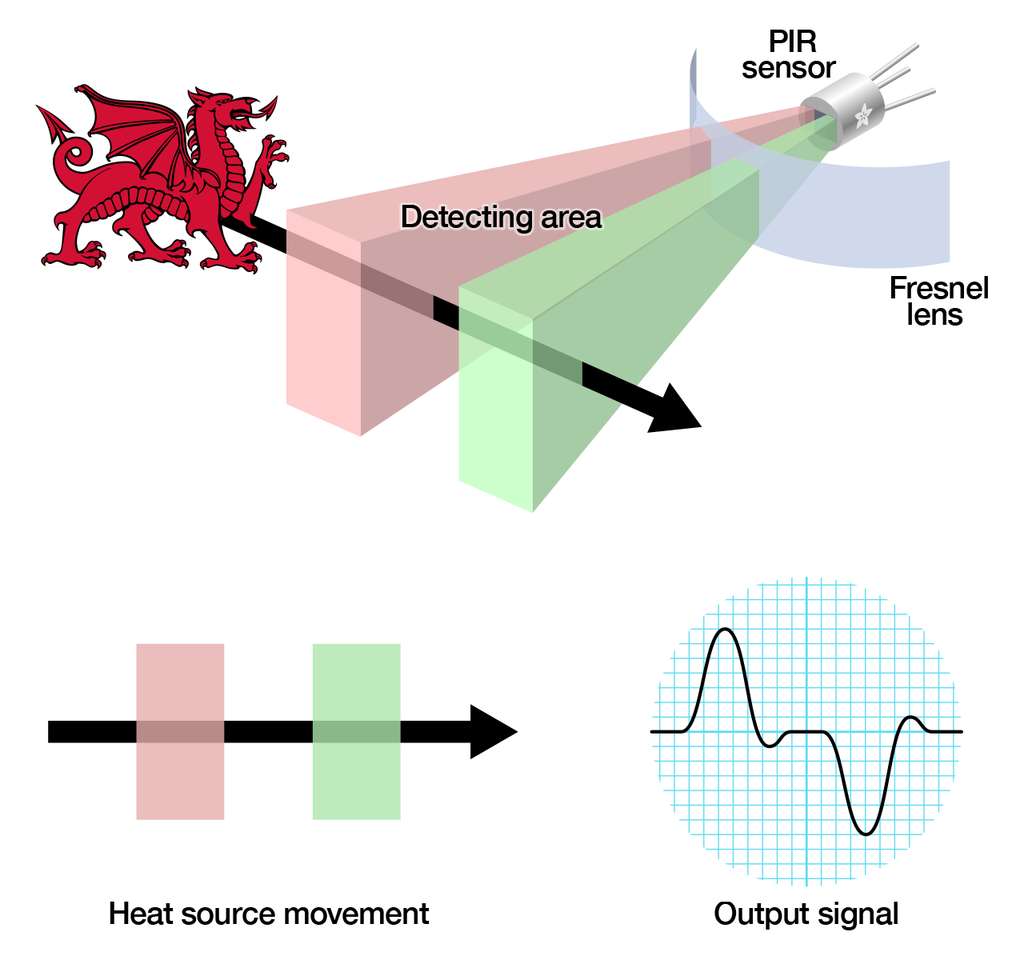
\includegraphics[scale=0.15]{pir4}
	\end{center}
	\caption{PIR Sensor Funktionsweise}
\end{figure}

\subsection{Implementierung im Projekt}
TODO
\begin{figure}
	\begin{center}
		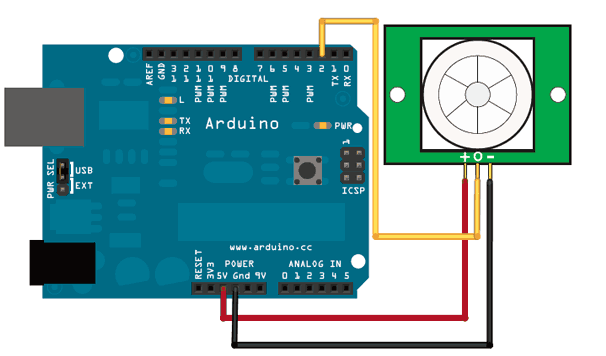
\includegraphics[scale=0.35]{pir5}
	\end{center}
	\caption{PIR Sensor Funktionsweise}
\end{figure}

\begin{lstlisting}[style=CStyle]
int inputPin = 2;	// choose the input pin (for PIR sensor)
int pirState = LOW;	// we start, assuming no motion detected
int val = 0;	// variable for reading the pin status

void setup()
{
	pinMode(inputPin, INPUT);	// declare sensor as input
	
}

void loop()
{
	val = digitalRead(inputPin);	// read input value
	if (val == HIGH)
	{
		lcd.backlight();
		lcd1.backlight();
		if (pirState == LOW)
		{
			// we have just turned on
			Serial.println("Motion detected!");
			// We only want to print on the output change, not state
			pirState = HIGH;
		}
	}
	else
	{
		lcd.noBacklight();
		lcd1.noBacklight();
		if (pirState == HIGH)
		{
			// we have just turned of
			Serial.println("Motion ended!");
			// We only want to print on the output change, not state
			pirState = LOW;
		}
	}
}
\end{lstlisting}

\begin{thebibliography}{00}
\bibitem{b1} https://github.com/adafruit/DHT-sensor-library
\bibitem{b2} https://github.com/semestrinis/Arduino/wiki/DHT22-temperature-humidity-sensor
\bibitem{b3} https://learn.adafruit.com/pir-passive-infrared-proximity-motion-sensor/overview
\bibitem{b4} https://learn.adafruit.com/pir-passive-infrared-proximity-motion-sensor/how-pirs-work
\bibitem{b5} https://learn.adafruit.com/pir-passive-infrared-proximity-motion-sensor/connecting-to-a-pir
\bibitem{b6}
\bibitem{b7}
\end{thebibliography}
\vspace{12pt}


\end{document}
